\chapter{How to Build a Fictional World --- Kate Messner}

This lecture begins in the right place: not with a definition, but with a collection of worlds that already work. Gandalf can die and return. The Matrix can download competence. Quidditch ends when the Snitch is caught. The answer to the ultimate question is \(42\). Only after that quick parade does Messner tell us what the examples were doing. They were all showing us that a fictional world becomes memorable not because anything can happen, but because what can happen is governed by rules. From there the lecture moves in a deliberate order: first consistency, then contrast with ordinary reality, then the reader's relation to the book-world, then the deeper puzzle of how marks on a page become lived experience, and finally the practical method by which a writer can build such a world and release characters into it.

\section{Rule-Bound Worlds}

Messner opens by stacking examples rather than explaining them. That rhythm matters. Before we are told what a fictional world is, we are shown that every durable one has a grammar of possibility. Gandalf's mixed mortality is not random. The Matrix does not grant skills by whim; it has a mechanism. Quidditch has an end condition. Even a line like ``the answer is \(42\)'' works because it sounds like the output of a world with its own strange but stable logic.

A compact way to record the lecture's opening examples is
\begin{align}
\text{mortal body} + \text{immortal spirit} &\Rightarrow \text{Gandalf can die and return},\\
\text{link up} + \text{hack code} &\Rightarrow \text{learn helicopter flight in seconds},\\
\text{Snitch caught} &\iff \text{Quidditch match ends},\\
\text{ultimate answer} &= 42.
\end{align}
These are not equations in the physicist's sense. They are note-form statements of local law. Messner's point is that a reader can learn them because they recur, constrain outcomes, and give the world a stable shape.

That is why she can then pivot so cleanly to the lecture's first general claim:
\begin{equation}
\text{consistent rules} \Rightarrow \text{believability} + \text{comprehensibility} + \text{explorability}.
\end{equation}
A world that is merely surprising is not yet a world. A world becomes explorable when we can infer, from one case to the next, what its boundaries are and what sorts of consequences its laws will produce.

\subsection{Question \& Answer}

\paragraph{Question.} What makes an invented world feel coherent rather than random?

\paragraph{Answer.} Coherence comes from regularity. The wonders may be extraordinary, but they must not be arbitrary. Once a reader can learn the world's constraints, the world stops being a bag of tricks and becomes a domain one can inhabit.

\section{Real Laws, Page Laws, and What Authors Build}

Messner's next move is especially sharp because it takes a grand idea and reduces it to one clean contrast. In real life, gravity holds the Harry Potter books to their shelves. The physical object in our world obeys our law. But on the pages of the fiction, after ``wizard,'' ``wand,'' and ``Wingardium Leviosa,'' that same law can be suspended or rewritten. The important distinction is not between order and disorder; it is between one lawful domain and another.

A convenient shorthand for the lecture's phrase ``a spectrum of physical and societal rules'' is
\begin{equation}
W = (R_{\mathrm{phys}},\,R_{\mathrm{soc}}),
\end{equation}
where \(W\) denotes the fictional world, \(R_{\mathrm{phys}}\) its physical rules, and \(R_{\mathrm{soc}}\) its social rules. This is editorial notation, not lecture notation, but it expresses the lecture's real structure accurately. The world is not a backdrop. It is a coupled system of constraints.

The gravity example may then be written schematically as
\begin{equation}
g_{\text{real world}} \neq g_{\text{wizarding page-world}}.
\end{equation}
Again, we should read this cautiously. Messner does not speak in symbols. She speaks in contrasts. But the symbolic form helps us see the point: worldbuilding is the controlled modification of law, not the abolition of law.

From here the lecture widens. Authors of science fiction and fantasy do not simply place a plot into a ready-made container. They build the container itself. They specify not only rules, but the larger infrastructure that lets those rules become a civilization:
\begin{equation}
\text{rules} \to \text{maps} \to \text{lineages} \to \text{languages} \to \text{cultures} \to \text{universes}.
\end{equation}
The arrow here indicates growth in articulated structure. A single rule may give us a gimmick. A system of rules, histories, and institutions gives us a world.

\section{When the Reader Understands the Book-World}

Messner then states the first major payoff of all this labor. When worldbuilding is done well, readers can understand the fictional world and its rules as well as the characters who live there do, and sometimes even better than they understand the world outside the book. This is a strong claim, and the lecture knows it is strong. It is why the next question must be ``But how?''

A compact way to write the claim is
\begin{equation}
\text{reader's grasp of book-world} \gtrsim \text{reader's grasp of outside world}.
\end{equation}
The symbol \(\gtrsim\) is only a shorthand for Messner's phrase ``just as well or even better.'' The lecture itself stays verbal. But the comparison is real, and it deserves to be written down.

The lecture also supplies a visual form of this comparison. The reader sits with the open book in the foreground; a small world begins to emerge from the pages; the outside world is represented as a separate social field behind it. The effect is not that reality disappears. It is that the book-world becomes, for a time, the more legible domain.

\begin{figure}[h]
\centering

\includegraphics[width=0.82\textwidth]{lecture_09_figure_03.png}
\caption{Reader, book-world, and the world outside the book.}
\end{figure}

We can also redraw the lecture's image as a cleaner schematic. The redraw is not meant to replace the original picture. It is meant to extract the structure that the picture implies.

\begin{figure}[h]
\centering
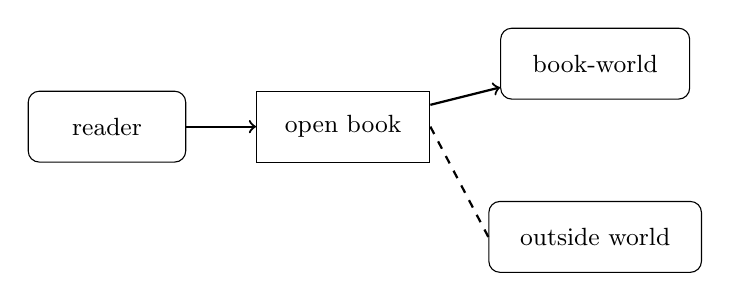
\begin{tikzpicture}[x=1cm,y=1cm]
\node[draw, rounded corners, minimum width=2.0cm, minimum height=0.9cm] (reader) at (0,0) {\small reader};
\node[draw, minimum width=2.2cm, minimum height=0.9cm] (book) at (3.0,0) {\small open book};
\node[draw, rounded corners, minimum width=2.4cm, minimum height=0.9cm] (inside) at (6.2,0.8) {\small book-world};
\node[draw, rounded corners, minimum width=2.7cm, minimum height=0.9cm] (outside) at (6.2,-1.4) {\small outside world};
\draw[->, thick] (reader) -- (book);
\draw[->, thick] (book) -- (inside);
\draw[dashed, thick] (book.east) -- (outside.west);
\end{tikzpicture}
\caption{A schematic reconstruction of the lecture's comparison between the world in the book and the world outside it.}
\end{figure}

\subsection{Question \& Answer}

\paragraph{Question.} How can a book-world become more legible than reality?

\paragraph{Answer.} Because the world of the book is curated. Its rules, histories, and consequences are selected, repeated, and made mutually intelligible. Reality is denser and noisier. A well-built fictional world can therefore become, for the reader, the more tractable system.

\section{How Squiggles Become Worlds}

Now the lecture stops and asks its deepest question. If readers really can inhabit such worlds, how does that happen? Messner's formulation is beautifully concrete. How can human-made squiggles on a page reflect light into the eye, become signals to the brain, and end as narrative strong enough to make us fight, cry, sing, think, or return to the real world altered?

The lecture's chain may be written as
\begin{equation}
\text{squiggles on page} \to \text{signals to the brain} \to \text{decoded narrative} \to \text{emotion/thought/action} \to \text{changed perspective}.
\end{equation}
This is not a completed theory of mind. It is a functional map. The lecture is deliberately not pretending to solve the full problem of reading. But it does insist that the transformation from page to world has stages, and that those stages culminate in both immersion and return.

\paragraph{Worked derivation.} If we unpack the lecture's chain step by step, we get the following narrative mechanism.
\begin{enumerate}
\item We begin with visible marks on a page.
\item Light from those marks reaches the eyes.
\item The nervous system converts that input into signals.
\item The mind decodes patterned signals as narrative order.
\item Narrative recruits feeling, thought, and imaginative participation.
\item The reader temporarily inhabits the fictional domain.
\item On returning to ordinary life, the reader's perspective may have shifted.
\end{enumerate}
Messner is careful here. She does not say that every step is fully understood. On the contrary, the lecture pauses to admit that perhaps no one yet knows the whole answer. But that admission does not stop the lecture. It becomes the bridge to practice.

\subsection{Question \& Answer}

\paragraph{Question.} How do marks on a page become a lived world in the reader's mind?

\paragraph{Answer.} The lecture gives us not a final explanation but a chain. Marks become signals, signals become decoded pattern, decoded pattern becomes story, and story recruits emotion and imagination strongly enough to restructure perception. The exact mechanism remains partly mysterious; the functional sequence is clear.

\section{From Mystery to Method}

Because the full mystery cannot be solved on the spot, Messner changes register. The lecture now says, in effect, that even if we cannot explain the whole alchemy of reading, we can still practice the craft that makes it possible. The tools she emphasizes are imagination and the willingness to live inside imagination long enough for a world to acquire thickness.

The first concrete step is historical. We do not begin by scattering decorative details. We begin by asking how the world came to be:
\begin{equation}
\text{past events} \to \text{timeline} \to \text{present structure of the world}.
\end{equation}
This is an important move. A timeline is not an appendix. It is the first answer to the question of why the world is arranged as it now is.

From there the lecture turns to a systematic questionnaire. At the macro level, we ask about the world's governing state:
\begin{equation}
(\text{rules},\ \text{government},\ \text{power},\ \text{beliefs},\ \text{values}).
\end{equation}
At the level of lived texture, we descend into daily life:
\begin{equation}
(\text{weather},\ \text{home/work/school},\ \text{food},\ \text{play},\ \text{young/old},\ \text{plants/animals},\ \text{technology},\ \text{transportation},\ \text{communication},\ \text{information}).
\end{equation}
This ordering matters. We move from law and power to habit and sensation. A world is not finished when we know its constitution. It is finished only when we know how it feels to live there.

\paragraph{Worked example.} Messner's practical method can be read as a disciplined expansion of the world state.
\begin{enumerate}
\item Specify the world's past and arrange it into a timeline.
\item Ask what physical and social rules are in force.
\item Ask who governs, who has power, and what people believe.
\item Ask what the society values and how violations are punished.
\item Ask how ordinary life is organized: weather, work, school, food, play, age, ecology, and technology.
\item Continue until the world is no longer merely described but inhabitable.
\end{enumerate}
The point is not to answer questions mechanically. The point is to ask enough of the right questions that the world begins to answer back.

\section{From World to Story}

The final movement of the lecture is as important as the opening. Worldbuilding is not the goal. Story is. Once we know the world as well as we hope the reader will know it, we set characters free in it and ask what follows. The world now ceases to be background and becomes a shaping force.

Messner's last compression can be written as
\begin{equation}
\text{world} + \text{characters} \Rightarrow \text{shaped individuals} \Rightarrow \text{conflict} \Rightarrow \text{story}.
\end{equation}
This is the lecture's true endpoint. The world exerts pressure. Characters absorb that pressure differently. Their wants, fears, permissions, prohibitions, and opportunities are all functions of the world they inhabit. Conflict is therefore not pasted onto the world after the fact. It emerges from the world once agents begin moving inside it.

We can say the same thing in ordinary prose. A world with rules but no people gives us a dossier. People with desires but no constraining world give us abstractions. Story appears when structured people meet a structured world under pressure.

\subsection{Question \& Answer}

\paragraph{Question.} When does worldbuilding stop being background and start becoming story?

\paragraph{Answer.} It becomes story the moment the world's rules begin shaping choice. Once characters are placed inside the world and must live under its laws, values, punishments, and possibilities, conflict appears. At that point the world is no longer scenery; it is an active term in the drama.

\section{Summary}

Messner's lecture gives us a small but precise mathematics of fictional worlds. First, every strong invented world is governed by consistent rules. Second, those rules may depart sharply from ordinary reality, but only in a controlled way. Third, when the construction is good enough, the reader can come to know the internal world of the book with remarkable clarity. Fourth, there is a real puzzle in how marks on a page produce that effect, even if the full mechanism remains partly mysterious. And fifth, the craft answer is practical: build the world's past, specify its laws and institutions, descend into daily life, and then let characters move inside the resulting structure. When that happens, worldbuilding ceases to be preparation and becomes story.